\documentclass{article}

\usepackage{polski}
\usepackage{amsmath}
\usepackage{graphicx}
\usepackage{float}
\usepackage{subfig}
\usepackage{multirow}

\title{Rozwiązywanie układów równań liniowych metodami iteracyjnymi}
\author{\textbf{Łukasz Wala}\\
    \textit{AGH, Wydział Informatyki, Elektroniki i Telekomunikacji} \\
    \textit{Metody Obliczeniowe w Nauce i Technice 2021/2022}}
\date{Kraków, \today}

\begin{document}
\maketitle

\section{Problem 1}
\subsection{Opis problemu}
Dany jest układ równań liniowych \textbf{Ax}=\textbf{b}.
Elementy macierzy \textbf{A} o wymiarze $n$\,x\,$n$ są określone wzorem:
$$
\begin{cases}
    a_{i,i}=k\\
    a_{i,j}=\frac{1}{|i-j|+m} \ dla \ i \ne j
\end{cases}i,j=1,...,n
$$

Gdzie $k=8$, $m=3$.

Za wektor \textbf{x} przyjęta zostanie dowolna $n$-elementowa permutacja ze zbioru \{1,-1\} i obliczony zostanie
wektor \textbf{b}. Układ zostanie rozwiązany metodą Jakobiego. Obliczenia zostaną wykonane dla różnych $n$,
dla różnych wektorów początkowych oraz różnych wartości $\rho$ w kryteriach stopu. Wyznaczone zostaną: liczba iteracji,
różnica w czasie obliczeń dla obu kryteriów stopu. Sprawdzona zostanie dokładność obliczeń.

Użyte kryteria stopu (norma euklidesowa):
\begin{enumerate}
    \item 
    $\left\|x^{(i+1)}-x^{(i)}\right\| < \rho$
    \item
    $\left\|Ax^{(i)}-b\right\| < \rho$
\end{enumerate}

\subsection{Opracowanie problemu}
Program użyty do rozwiązania układu został napisany w języku Python z użyciem pakietu numpy. Poniżej tabele zależności
liczby $n$ oraz precyzji (błąd wyniku, liczba iteracji oraz czas obliczeń) dla wektora początkowego zawierającego same
zera:

\newpage
\thispagestyle{empty}

\begin{table}[H]
\centering
\begin{tabular}{|l|l|l|l|l|l|}
\hline
& 0.01 & 0.001 & 0.0001 & 0.00001 & 0.000001 \\ \hline
3 & 1.21461e-04 & 6.45239e-06 & 3.63832e-07 & 3.63832e-07 & 2.10000e-08 \\ \hline
6 & 9.67915e-05 & 3.33425e-06 & 3.33425e-06 & 1.15019e-07 & 3.97211e-09 \\ \hline
9 & 2.49465e-04 & 4.35374e-05 & 7.59930e-06 & 1.32644e-06 & 4.04122e-08 \\ \hline
12 & 1.44833e-04 & 5.06499e-06 & 1.77686e-07 & 1.77686e-07 & 6.25783e-09 \\ \hline
15 & 7.74528e-04 & 1.94437e-04 & 1.22542e-05 & 7.72308e-07 & 1.93885e-07 \\ \hline
18 & 2.17354e-04 & 1.19462e-05 & 8.61069e-07 & 6.84378e-08 & 6.84378e-08 \\ \hline
21 & 1.42965e-03 & 1.36194e-04 & 1.29746e-05 & 1.23603e-06 & 1.17750e-07 \\ \hline
24 & 3.61263e-04 & 3.51678e-05 & 4.00609e-06 & 4.64506e-07 & 5.39479e-08 \\ \hline
27 & 2.13243e-03 & 9.54138e-05 & 1.20256e-05 & 1.51565e-06 & 1.91026e-07 \\ \hline
30 & 5.61660e-04 & 7.53908e-05 & 1.09908e-05 & 2.36099e-07 & 3.46098e-08 \\ \hline
33 & 1.11982e-03 & 1.73729e-04 & 2.69524e-05 & 1.64697e-06 & 2.55512e-07 \\ \hline
36 & 7.94304e-04 & 1.30859e-04 & 3.93942e-06 & 6.84350e-07 & 1.18885e-07 \\ \hline
39 & 1.51382e-03 & 2.76484e-04 & 2.15806e-05 & 1.68445e-06 & 1.31478e-07 \\ \hline
42 & 1.04374e-03 & 3.94455e-05 & 7.81636e-06 & 1.54897e-06 & 6.08309e-08 \\ \hline
45 & 1.92798e-03 & 1.83768e-04 & 1.75161e-05 & 1.66958e-06 & 1.59139e-07 \\ \hline
48 & 2.78556e-04 & 6.13257e-05 & 1.35159e-05 & 6.56653e-07 & 1.44739e-07 \\ \hline
51 & 2.35451e-03 & 2.65404e-04 & 2.99170e-05 & 1.62904e-06 & 1.83629e-07 \\ \hline
54 & 3.66503e-04 & 8.81516e-05 & 5.11145e-06 & 1.23096e-06 & 7.13909e-08 \\ \hline
57 & 2.78791e-03 & 1.83892e-04 & 2.39349e-05 & 3.11529e-06 & 2.05489e-07 \\ \hline
60 & 4.61435e-04 & 1.19642e-04 & 8.06467e-06 & 5.43773e-07 & 1.41200e-07 \\ \hline
63 & 3.22426e-03 & 2.51372e-04 & 1.95981e-05 & 2.89158e-06 & 2.25441e-07 \\ \hline
66 & 5.61897e-04 & 1.55462e-04 & 1.19379e-05 & 9.17095e-07 & 7.04549e-08 \\ \hline
69 & 2.00711e-03 & 3.30835e-04 & 2.98998e-05 & 2.70225e-06 & 2.44220e-07 \\ \hline
72 & 6.66686e-04 & 1.95256e-04 & 1.68111e-05 & 1.44822e-06 & 1.24764e-07 \\ \hline
75 & 2.32069e-03 & 2.39331e-04 & 2.46822e-05 & 2.54547e-06 & 2.62514e-07 \\ \hline
78 & 7.74815e-04 & 7.36645e-05 & 2.27467e-05 & 2.16950e-06 & 2.06929e-07 \\ \hline
81 & 2.64250e-03 & 3.06970e-04 & 3.56599e-05 & 2.41844e-06 & 2.80944e-07 \\ \hline
84 & 8.85472e-04 & 9.21784e-05 & 9.63016e-06 & 1.00635e-06 & 1.05165e-07 \\ \hline
87 & 2.97092e-03 & 2.30665e-04 & 2.98580e-05 & 2.31823e-06 & 3.00079e-07 \\ \hline
90 & 9.97994e-04 & 1.12765e-04 & 1.27944e-05 & 1.45212e-06 & 1.64816e-07 \\ \hline
93 & 3.30457e-03 & 2.90377e-04 & 2.55162e-05 & 3.64670e-06 & 3.20445e-07 \\ \hline
96 & 1.11184e-03 & 1.35356e-04 & 1.65563e-05 & 2.02592e-06 & 2.47912e-07 \\ \hline
99 & 3.64231e-03 & 3.58681e-04 & 3.53223e-05 & 3.47848e-06 & 3.42554e-07 \\ \hline
102 & 1.22655e-03 & 1.59873e-04 & 2.09496e-05 & 9.94493e-07 & 1.30387e-07 \\ \hline
105 & 2.55887e-03 & 2.80012e-04 & 3.06413e-05 & 3.35303e-06 & 3.66916e-07 \\ \hline
108 & 1.34177e-03 & 1.86237e-04 & 2.60035e-05 & 1.35788e-06 & 1.89714e-07 \\ \hline
111 & 2.83436e-03 & 3.42094e-04 & 2.70507e-05 & 3.26492e-06 & 3.94063e-07 \\ \hline
114 & 1.45718e-03 & 2.14366e-04 & 1.22184e-05 & 1.81055e-06 & 2.68296e-07 \\ \hline
117 & 3.11676e-03 & 2.75045e-04 & 3.63767e-05 & 3.21016e-06 & 2.83290e-07 \\ \hline
120 & 1.57255e-03 & 2.44177e-04 & 1.51069e-05 & 2.36451e-06 & 1.46424e-07 \\ \hline
123 & 3.40539e-03 & 3.33059e-04 & 3.25747e-05 & 3.18595e-06 & 3.11601e-07 \\ \hline
126 & 1.68767e-03 & 2.75590e-04 & 1.84064e-05 & 1.23060e-06 & 2.02718e-07 \\ \hline
129 & 3.69962e-03 & 3.98547e-04 & 2.96161e-05 & 3.19046e-06 & 3.43701e-07 \\ \hline
132 & 1.80236e-03 & 1.28150e-04 & 2.21372e-05 & 1.59022e-06 & 2.74807e-07 \\ \hline
135 & 3.99890e-03 & 3.30473e-04 & 3.89961e-05 & 3.22272e-06 & 3.80284e-07 \\ \hline
138 & 1.91649e-03 & 1.45657e-04 & 2.63179e-05 & 2.02251e-06 & 1.55438e-07 \\ \hline
141 & 3.05692e-03 & 3.93150e-04 & 3.59237e-05 & 3.28249e-06 & 2.99934e-07 \\ \hline
144 & 2.02995e-03 & 1.64273e-04 & 1.34468e-05 & 2.53591e-06 & 2.07692e-07 \\ \hline
147 & 3.32050e-03 & 3.33699e-04 & 3.35358e-05 & 3.37026e-06 & 3.38701e-07 \\ \hline
\end{tabular}
\caption{Błędy obliczeń (wiersze - $n$, kolumny - precyzja, kryterium stopu 1)}
\end{table}

Jak nietrudno było się domyślić, błąd rozwiązania maleje wraz ze malejącą wartością $\rho$ niezależnie od rozmiaru
macierzy. Ciężko na pierwszy rzut oka zauważyć zależność $n$ oraz błędu (), jednak może być to spowodowane faktem, że program
działa aż do uzyskania pewnej dokładności określonej przez kryteria stopu, więc uzyskanie tej samej dokładności dla 
dużych macierzy wymaga więcej iteracji lub czasu, co zostanie zbadane później.

\begin{figure}[H]
    \centering
    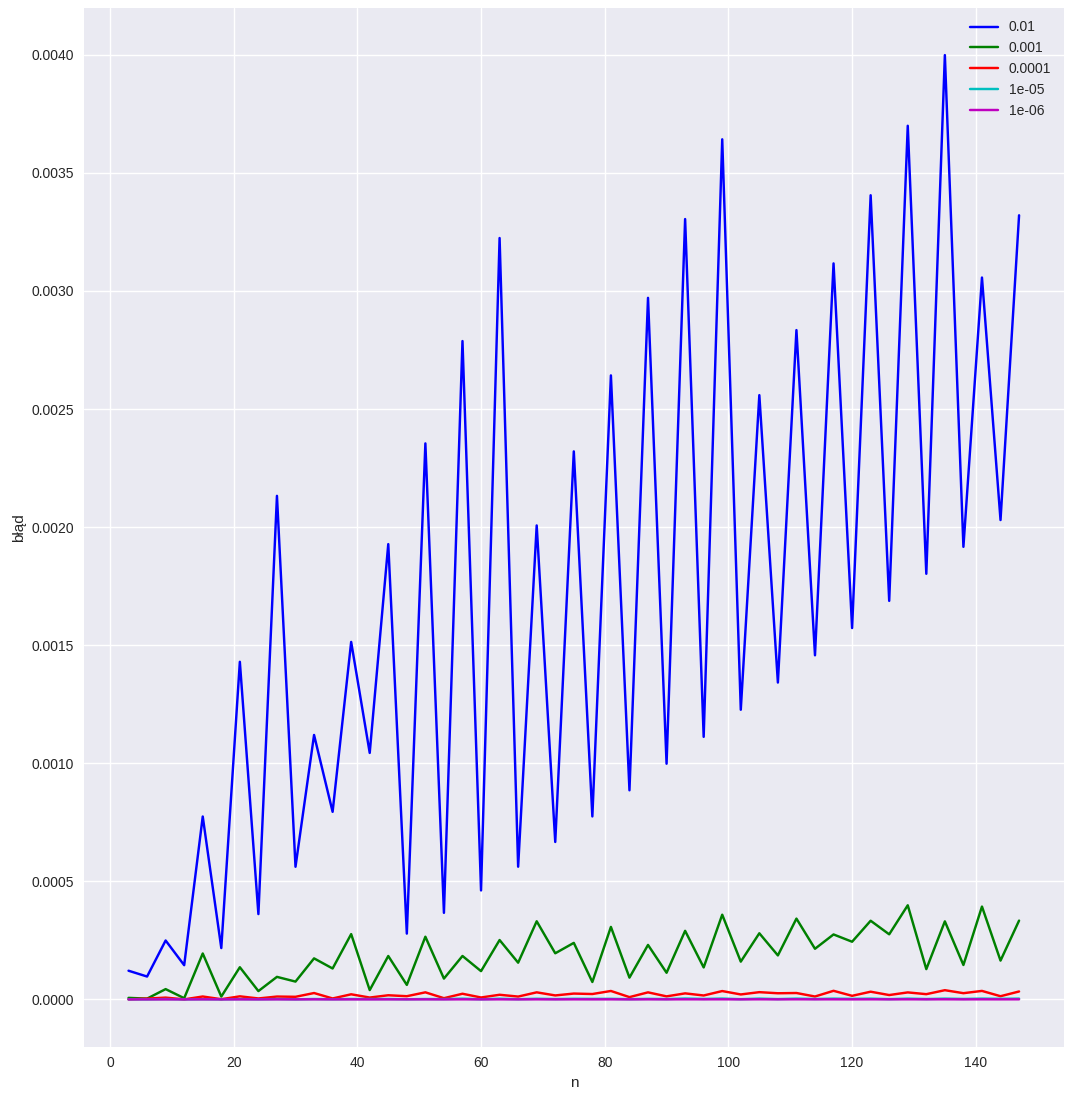
\includegraphics[width=\textwidth]{img/plot_1.png}
    \caption{Wykres błędów na podstawie powyższej tabeli}
\end{figure}

Poniżej tabela błędów dla kryterium 2, można w niej zauważyć, że generalnie wyniki są odrobinę bardziej dokładne,
co oznacza że kryterium 2 jest bardziej rygorystyczne, lecz zapewne wymaga więszej liczby iteracji/czasu.

\newpage
\thispagestyle{empty}

\begin{table}[H]
\centering
\begin{tabular}{|l|l|l|l|l|l|}
\hline
& 0.01 & 0.001 & 0.0001 & 0.00001 & 0.000001 \\ \hline
3 & 1.21461e-04 & 6.45239e-06 & 6.45239e-06 & 3.63832e-07 & 2.10000e-08 \\ \hline
6 & 9.67915e-05 & 9.67915e-05 & 3.33425e-06 & 1.15019e-07 & 1.15019e-07 \\ \hline
9 & 2.49465e-04 & 4.35374e-05 & 7.59930e-06 & 2.31526e-07 & 4.04122e-08 \\ \hline
12 & 1.44833e-04 & 5.06499e-06 & 5.06499e-06 & 1.77686e-07 & 6.25783e-09 \\ \hline
15 & 7.74528e-04 & 4.88126e-05 & 3.07636e-06 & 7.72308e-07 & 4.86740e-08 \\ \hline
18 & 2.17354e-04 & 1.19462e-05 & 8.61069e-07 & 8.61069e-07 & 6.84378e-08 \\ \hline
21 & 4.41258e-04 & 4.20365e-05 & 4.00461e-06 & 3.81500e-07 & 3.63436e-08 \\ \hline
24 & 3.61263e-04 & 3.51678e-05 & 4.00609e-06 & 4.64506e-07 & 5.39479e-08 \\ \hline
27 & 7.57038e-04 & 3.38734e-05 & 4.26925e-06 & 5.38078e-07 & 6.78171e-08 \\ \hline
30 & 5.61660e-04 & 7.53908e-05 & 1.61063e-06 & 2.36099e-07 & 3.46098e-08 \\ \hline
33 & 4.41073e-04 & 6.84282e-05 & 4.18141e-06 & 6.48707e-07 & 3.96402e-08 \\ \hline
36 & 7.94304e-04 & 2.26793e-05 & 3.93942e-06 & 6.84350e-07 & 2.06526e-08 \\ \hline
39 & 6.46953e-04 & 5.04971e-05 & 3.94149e-06 & 7.19874e-07 & 5.61889e-08 \\ \hline
42 & 1.04374e-03 & 3.94455e-05 & 7.81636e-06 & 3.06961e-07 & 6.08309e-08 \\ \hline
45 & 4.02297e-04 & 8.39446e-05 & 8.00132e-06 & 7.62659e-07 & 7.26941e-08 \\ \hline
48 & 2.78556e-04 & 6.13257e-05 & 2.97912e-06 & 6.56653e-07 & 3.19033e-08 \\ \hline
51 & 5.49420e-04 & 6.19319e-05 & 6.98111e-06 & 7.86927e-07 & 4.28497e-08 \\ \hline
54 & 3.66503e-04 & 8.81516e-05 & 5.11145e-06 & 2.96444e-07 & 7.13909e-08 \\ \hline
57 & 7.16009e-04 & 4.72290e-05 & 6.14718e-06 & 8.00098e-07 & 5.27756e-08 \\ \hline
60 & 4.61435e-04 & 3.10593e-05 & 8.06467e-06 & 5.43773e-07 & 3.66652e-08 \\ \hline
63 & 4.75711e-04 & 7.01884e-05 & 5.47220e-06 & 8.07391e-07 & 6.29478e-08 \\ \hline
66 & 5.61897e-04 & 4.30739e-05 & 3.30878e-06 & 9.17095e-07 & 7.04549e-08 \\ \hline
69 & 6.03390e-04 & 5.45324e-05 & 4.92846e-06 & 4.45418e-07 & 7.34192e-08 \\ \hline
72 & 6.66686e-04 & 5.72821e-05 & 4.93413e-06 & 4.25072e-07 & 3.66201e-08 \\ \hline
75 & 7.45259e-04 & 7.68584e-05 & 7.92640e-06 & 4.63240e-07 & 4.77739e-08 \\ \hline
78 & 7.74815e-04 & 7.36645e-05 & 7.02477e-06 & 6.70024e-07 & 6.39078e-08 \\ \hline
81 & 5.25806e-04 & 6.10815e-05 & 7.09568e-06 & 4.81226e-07 & 5.59028e-08 \\ \hline
84 & 8.85472e-04 & 9.21784e-05 & 3.11306e-06 & 3.25318e-07 & 3.39963e-08 \\ \hline
87 & 6.41126e-04 & 4.97784e-05 & 6.44345e-06 & 5.00283e-07 & 6.47580e-08 \\ \hline
90 & 3.35039e-04 & 3.79800e-05 & 4.31031e-06 & 4.89216e-07 & 5.55261e-08 \\ \hline
93 & 7.68105e-04 & 6.74955e-05 & 5.93101e-06 & 5.21175e-07 & 7.44846e-08 \\ \hline
96 & 3.87378e-04 & 4.73334e-05 & 5.79147e-06 & 7.08696e-07 & 8.67234e-08 \\ \hline
99 & 5.70218e-04 & 5.61541e-05 & 5.52995e-06 & 5.44580e-07 & 5.36292e-08 \\ \hline
102 & 4.42118e-04 & 5.78648e-05 & 7.58536e-06 & 3.60095e-07 & 4.72117e-08 \\ \hline
105 & 6.78461e-04 & 7.42429e-05 & 5.21928e-06 & 5.71138e-07 & 6.24987e-08 \\ \hline
108 & 4.99013e-04 & 6.95788e-05 & 3.63282e-06 & 5.07552e-07 & 7.09120e-08 \\ \hline
111 & 5.22164e-04 & 6.30233e-05 & 4.98349e-06 & 6.01488e-07 & 7.25973e-08 \\ \hline
114 & 5.57838e-04 & 8.24736e-05 & 4.70338e-06 & 6.96966e-07 & 3.97575e-08 \\ \hline
117 & 6.17783e-04 & 5.45179e-05 & 7.21040e-06 & 6.36301e-07 & 5.61521e-08 \\ \hline
120 & 6.18388e-04 & 3.81869e-05 & 5.97660e-06 & 3.70102e-07 & 5.79298e-08 \\ \hline
123 & 7.22884e-04 & 7.07013e-05 & 6.91491e-06 & 6.76310e-07 & 6.61461e-08 \\ \hline
126 & 6.80479e-04 & 4.53541e-05 & 7.47041e-06 & 4.99464e-07 & 8.22776e-08 \\ \hline
129 & 5.77774e-04 & 6.22422e-05 & 6.70520e-06 & 7.22335e-07 & 5.36768e-08 \\ \hline
132 & 7.43944e-04 & 5.32575e-05 & 3.82537e-06 & 6.61062e-07 & 4.74895e-08 \\ \hline
135 & 6.73762e-04 & 5.56810e-05 & 6.57042e-06 & 5.42992e-07 & 6.40737e-08 \\ \hline
138 & 8.08630e-04 & 6.19079e-05 & 4.75706e-06 & 8.59896e-07 & 6.60863e-08 \\ \hline
141 & 5.53366e-04 & 7.11686e-05 & 6.50296e-06 & 5.94200e-07 & 5.42944e-08 \\ \hline
144 & 3.78654e-04 & 7.13134e-05 & 5.83947e-06 & 4.78252e-07 & 3.91692e-08 \\ \hline
147 & 6.43360e-04 & 6.46559e-05 & 6.49774e-06 & 6.53004e-07 & 6.56251e-08 \\ \hline
\end{tabular}
\caption{Błędy obliczeń (wiersze - $n$, kolumny - precyzja, kryterium stopu 2)}
\end{table}

\begin{figure}[H]
    \centering
    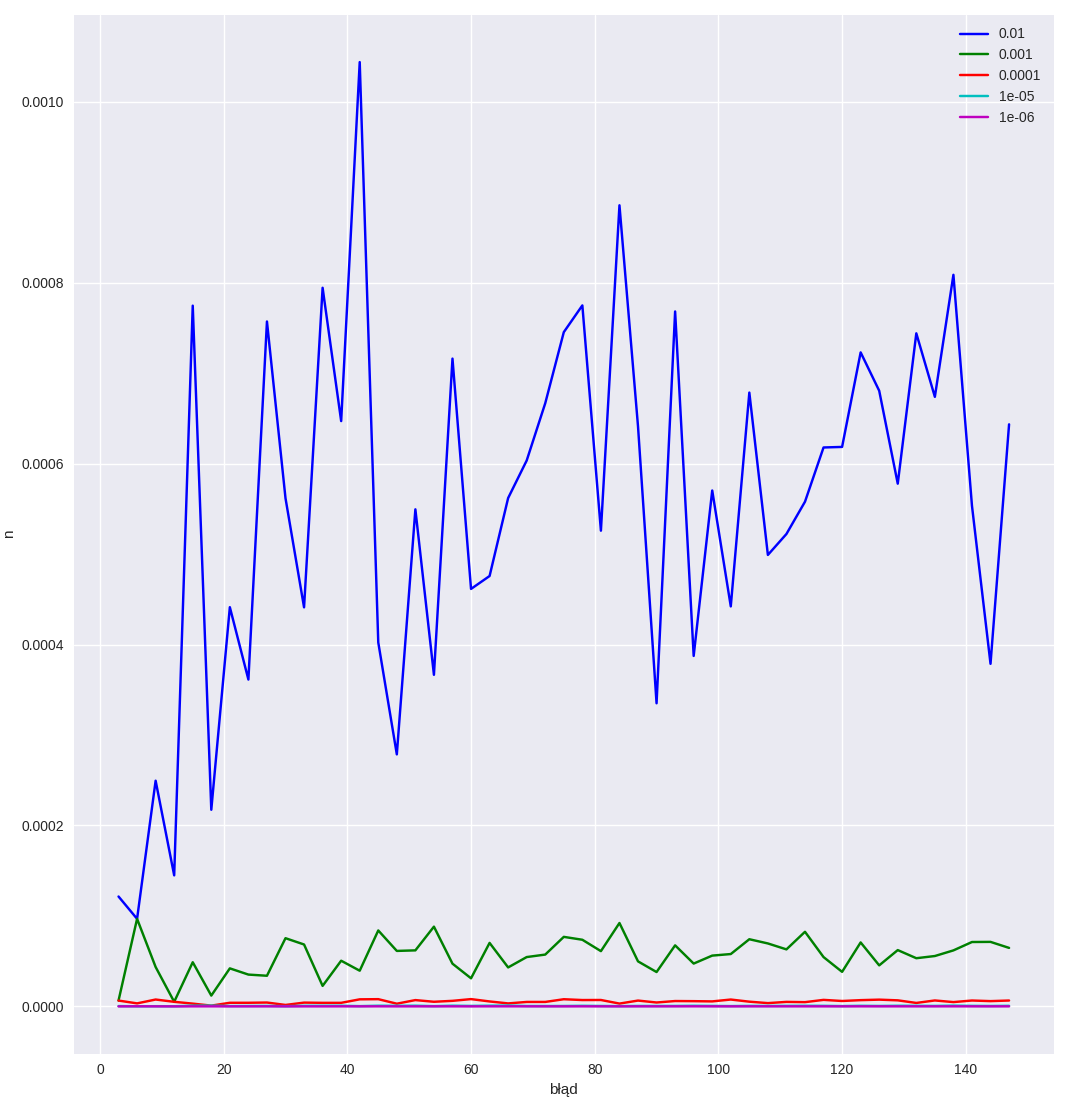
\includegraphics[width=\textwidth]{img/plot_2.png}
    \caption{Wykres błędów na podstawie powyższej tabeli}
\end{figure}

Teraz zbadane zostaną liczby iteracji/czas działania dla poszczególnych precyzji oraz wartości $n$.

\begin{table}[H]
\centering
\begin{tabular}{|l|l|l|l|l|l|}
\hline
& 0.01 & 0.001 & 0.0001 & 0.00001 & 0.000001 \\ \hline
3 & 3 & 4 & 5 & 5 & 6 \\ \hline
6 & 3 & 4 & 4 & 5 & 6 \\ \hline
9 & 4 & 5 & 6 & 7 & 9 \\ \hline
12 & 3 & 4 & 5 & 5 & 6 \\ \hline
15 & 4 & 5 & 7 & 9 & 10 \\ \hline
18 & 3 & 4 & 5 & 6 & 6 \\ \hline
21 & 4 & 6 & 8 & 10 & 12 \\ \hline
24 & 3 & 4 & 5 & 6 & 7 \\ \hline
27 & 4 & 7 & 9 & 11 & 13 \\ \hline
30 & 3 & 4 & 5 & 7 & 8 \\ \hline
33 & 5 & 7 & 9 & 12 & 14 \\ \hline
36 & 3 & 4 & 6 & 7 & 8 \\ \hline
39 & 5 & 7 & 10 & 13 & 16 \\ \hline
42 & 3 & 5 & 6 & 7 & 9 \\ \hline
45 & 5 & 8 & 11 & 14 & 17 \\ \hline
48 & 4 & 5 & 6 & 8 & 9 \\ \hline
51 & 5 & 8 & 11 & 15 & 18 \\ \hline
54 & 4 & 5 & 7 & 8 & 10 \\ \hline
57 & 5 & 9 & 12 & 15 & 19 \\ \hline
60 & 4 & 5 & 7 & 9 & 10 \\ \hline
63 & 5 & 9 & 13 & 16 & 20 \\ \hline
66 & 4 & 5 & 7 & 9 & 11 \\ \hline
69 & 6 & 9 & 13 & 17 & 21 \\ \hline
72 & 4 & 5 & 7 & 9 & 11 \\ \hline
75 & 6 & 10 & 14 & 18 & 22 \\ \hline
78 & 4 & 6 & 7 & 9 & 11 \\ \hline
81 & 6 & 10 & 14 & 19 & 23 \\ \hline
84 & 4 & 6 & 8 & 10 & 12 \\ \hline
87 & 6 & 11 & 15 & 20 & 24 \\ \hline
90 & 4 & 6 & 8 & 10 & 12 \\ \hline
93 & 6 & 11 & 16 & 20 & 25 \\ \hline
96 & 4 & 6 & 8 & 10 & 12 \\ \hline
99 & 6 & 11 & 16 & 21 & 26 \\ \hline
102 & 4 & 6 & 8 & 11 & 13 \\ \hline
105 & 7 & 12 & 17 & 22 & 27 \\ \hline
108 & 4 & 6 & 8 & 11 & 13 \\ \hline
111 & 7 & 12 & 18 & 23 & 28 \\ \hline
114 & 4 & 6 & 9 & 11 & 13 \\ \hline
117 & 7 & 13 & 18 & 24 & 30 \\ \hline
120 & 4 & 6 & 9 & 11 & 14 \\ \hline
123 & 7 & 13 & 19 & 25 & 31 \\ \hline
126 & 4 & 6 & 9 & 12 & 14 \\ \hline
129 & 7 & 13 & 20 & 26 & 32 \\ \hline
132 & 4 & 7 & 9 & 12 & 14 \\ \hline
135 & 7 & 14 & 20 & 27 & 33 \\ \hline
138 & 4 & 7 & 9 & 12 & 15 \\ \hline
141 & 8 & 14 & 21 & 28 & 35 \\ \hline
144 & 4 & 7 & 10 & 12 & 15 \\ \hline
147 & 8 & 15 & 22 & 29 & 36 \\ \hline
\end{tabular}
\caption{Iteracje (wiersze - $n$, kolumny - precyzja, kryterium stopu 1)}
\end{table}

Lepsza precyzja wymaga wicej iteracji, co jest zgodne z intuicją. Oprócz tego potwierdzają się wcześniejsze przypuszczenia
o tym, że przyczyną dobrej precyzji dla większych macierzy jest większa liczba iteracji. Można też zauważyć, że przyrost
liczby iteracji w zależności od $n$ jest większy dla lepszych precyzji.

Zgodnie z poprzednimi przypuszczeniami, liczba iteracji rośnie wraz ze wzrastającą precyzją. Co jednak bardzo zastawiające, 
przyrost jest jakby niezależny dla nieparzystych oraz parzystych wartości $n$, tzn. gdyby odseparować na osobnych wykresach
liczby iteracji dla wartości parzystych i nieparzystych $n$, oba te wykresy byłyby niemalejące. Podobne zjawisko występuje
dla drugiego kryterium stopu.

\begin{figure}[H]
    \centering
    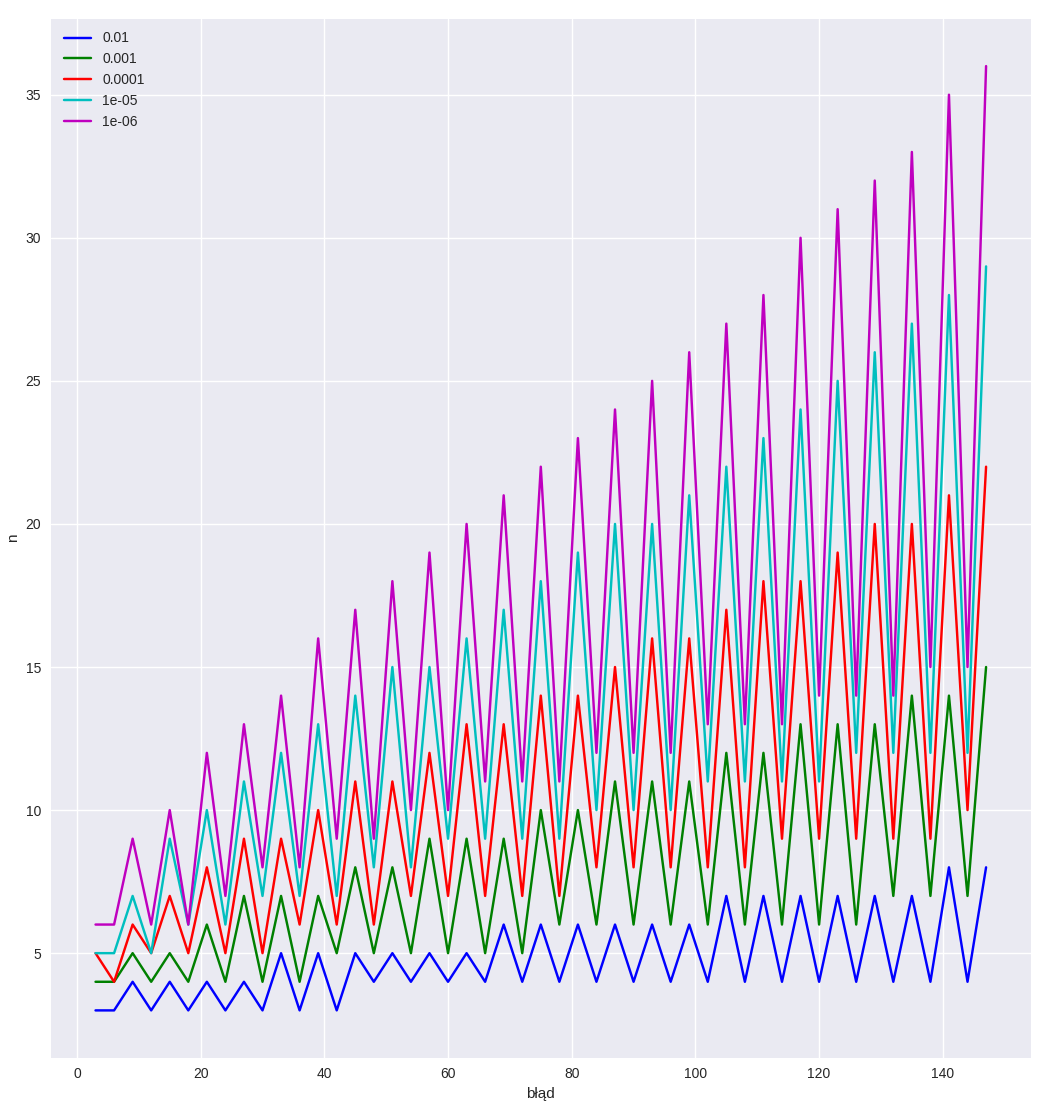
\includegraphics[width=\textwidth]{img/plot_3.png}
    \caption{Liczba iteracji na podstawie powyższej tabeli}
\end{figure}

\begin{table}[H]
\centering
\begin{tabular}{|l|l|l|l|l|l|}
\hline
& 0.01 & 0.001 & 0.0001 & 0.00001 & 0.000001 \\ \hline
3 & 3 & 4 & 4 & 5 & 6 \\ \hline
6 & 3 & 3 & 4 & 5 & 5 \\ \hline
9 & 4 & 5 & 6 & 8 & 9 \\ \hline
12 & 3 & 4 & 4 & 5 & 6 \\ \hline
15 & 4 & 6 & 8 & 9 & 11 \\ \hline
18 & 3 & 4 & 5 & 5 & 6 \\ \hline
21 & 5 & 7 & 9 & 11 & 13 \\ \hline
24 & 3 & 4 & 5 & 6 & 7 \\ \hline
27 & 5 & 8 & 10 & 12 & 14 \\ \hline
30 & 3 & 4 & 6 & 7 & 8 \\ \hline
33 & 6 & 8 & 11 & 13 & 16 \\ \hline
36 & 3 & 5 & 6 & 7 & 9 \\ \hline
39 & 6 & 9 & 12 & 14 & 17 \\ \hline
42 & 3 & 5 & 6 & 8 & 9 \\ \hline
45 & 7 & 9 & 12 & 15 & 18 \\ \hline
48 & 4 & 5 & 7 & 8 & 10 \\ \hline
51 & 7 & 10 & 13 & 16 & 20 \\ \hline
54 & 4 & 5 & 7 & 9 & 10 \\ \hline
57 & 7 & 11 & 14 & 17 & 21 \\ \hline
60 & 4 & 6 & 7 & 9 & 11 \\ \hline
63 & 8 & 11 & 15 & 18 & 22 \\ \hline
66 & 4 & 6 & 8 & 9 & 11 \\ \hline
69 & 8 & 12 & 16 & 20 & 23 \\ \hline
72 & 4 & 6 & 8 & 10 & 12 \\ \hline
75 & 8 & 12 & 16 & 21 & 25 \\ \hline
78 & 4 & 6 & 8 & 10 & 12 \\ \hline
81 & 9 & 13 & 17 & 22 & 26 \\ \hline
84 & 4 & 6 & 9 & 11 & 13 \\ \hline
87 & 9 & 14 & 18 & 23 & 27 \\ \hline
90 & 5 & 7 & 9 & 11 & 13 \\ \hline
93 & 9 & 14 & 19 & 24 & 28 \\ \hline
96 & 5 & 7 & 9 & 11 & 13 \\ \hline
99 & 10 & 15 & 20 & 25 & 30 \\ \hline
102 & 5 & 7 & 9 & 12 & 14 \\ \hline
105 & 10 & 15 & 21 & 26 & 31 \\ \hline
108 & 5 & 7 & 10 & 12 & 14 \\ \hline
111 & 11 & 16 & 22 & 27 & 32 \\ \hline
114 & 5 & 7 & 10 & 12 & 15 \\ \hline
117 & 11 & 17 & 22 & 28 & 34 \\ \hline
120 & 5 & 8 & 10 & 13 & 15 \\ \hline
123 & 11 & 17 & 23 & 29 & 35 \\ \hline
126 & 5 & 8 & 10 & 13 & 15 \\ \hline
129 & 12 & 18 & 24 & 30 & 37 \\ \hline
132 & 5 & 8 & 11 & 13 & 16 \\ \hline
135 & 12 & 19 & 25 & 32 & 38 \\ \hline
138 & 5 & 8 & 11 & 13 & 16 \\ \hline
141 & 13 & 19 & 26 & 33 & 40 \\ \hline
144 & 6 & 8 & 11 & 14 & 17 \\ \hline
147 & 13 & 20 & 27 & 34 & 41 \\ \hline
\end{tabular}
\caption{Iteracje (wiersze - $n$, kolumny - precyzja, kryterium stopu 2)}
\end{table}

\begin{figure}[H]
    \centering
    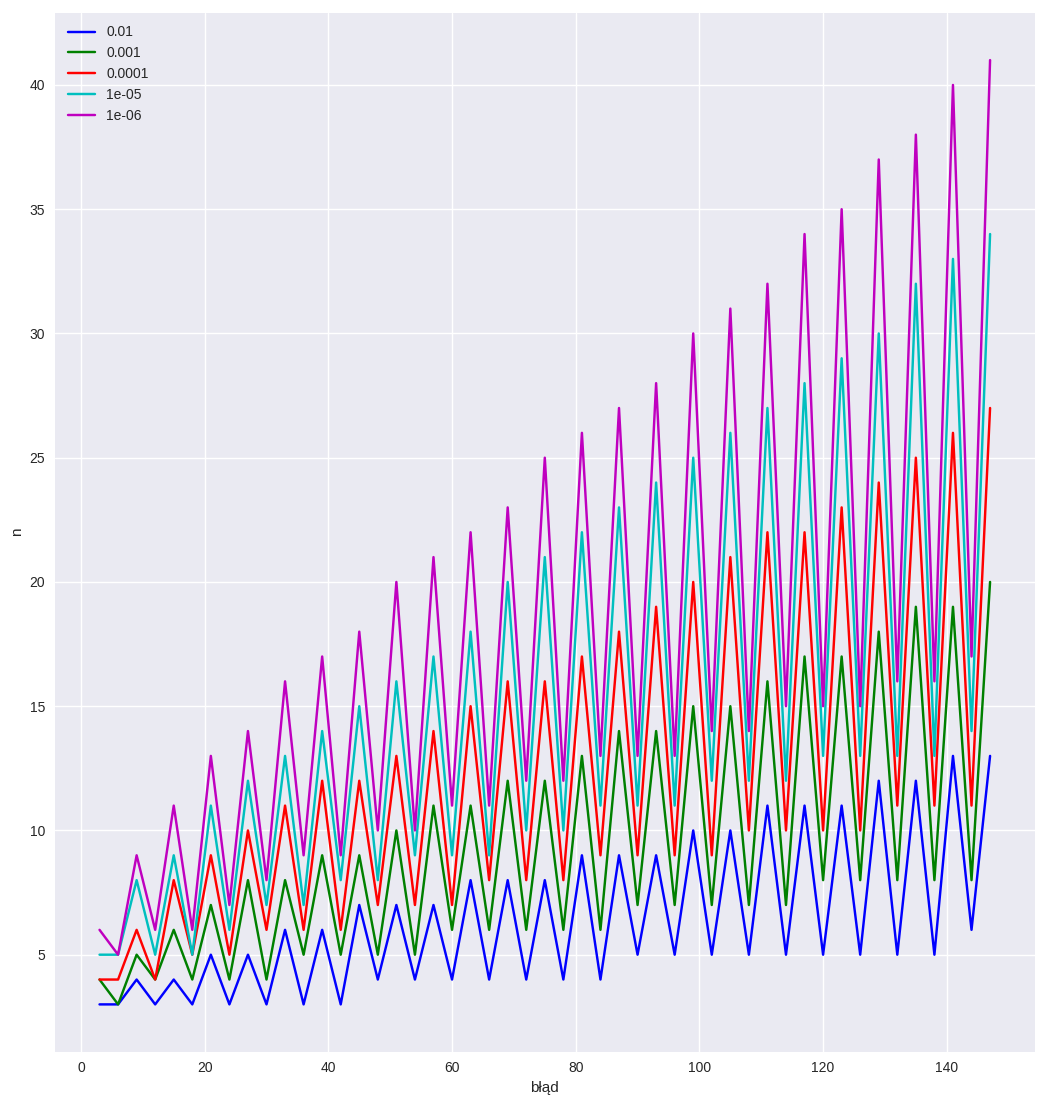
\includegraphics[width=\textwidth]{img/plot_4.png}
    \caption{Liczba iteracji na podstawie powyższej tabeli}
\end{figure}

W ogólności dla drugiego, bardziej rygorystycznego kryterium stopu potrzeba więcej iteracji.
Poniżej tabele czasu w sekundach:

\begin{table}[H]
\centering
\begin{tabular}{|l|l|l|l|l|l|}
\hline
& 0.01 & 0.001 & 0.0001 & 0.00001 & 0.000001 \\ \hline
3 & 0.0000875 & 0.0000467 & 0.0000496 & 0.0000479 & 0.0000532 \\ \hline
6 & 0.0000553 & 0.0000694 & 0.0000434 & 0.0000455 & 0.0000911 \\ \hline
9 & 0.0000851 & 0.0000927 & 0.0000794 & 0.0000591 & 0.0000679 \\ \hline
12 & 0.0000625 & 0.0000656 & 0.0000825 & 0.0000935 & 0.0000961 \\ \hline
15 & 0.0000772 & 0.0000820 & 0.0000939 & 0.0001132 & 0.0001304 \\ \hline
18 & 0.0000753 & 0.0000722 & 0.0000730 & 0.0000877 & 0.0000925 \\ \hline
21 & 0.0000985 & 0.0000927 & 0.0001428 & 0.0001245 & 0.0001514 \\ \hline
24 & 0.0000935 & 0.0001035 & 0.0001106 & 0.0001278 & 0.0001600 \\ \hline
27 & 0.0001264 & 0.0001535 & 0.0001547 & 0.0001626 & 0.0001926 \\ \hline
30 & 0.0002003 & 0.0001001 & 0.0001323 & 0.0001588 & 0.0000765 \\ \hline
33 & 0.0001099 & 0.0000854 & 0.0000761 & 0.0001080 & 0.0001056 \\ \hline
36 & 0.0000687 & 0.0000479 & 0.0000546 & 0.0000613 & 0.0000694 \\ \hline
39 & 0.0001190 & 0.0000687 & 0.0000811 & 0.0001004 & 0.0001278 \\ \hline
42 & 0.0000904 & 0.0000553 & 0.0000744 & 0.0000978 & 0.0000811 \\ \hline
45 & 0.0001194 & 0.0000758 & 0.0000896 & 0.0001173 & 0.0001295 \\ \hline
48 & 0.0000827 & 0.0000536 & 0.0000563 & 0.0001314 & 0.0000889 \\ \hline
51 & 0.0000858 & 0.0001590 & 0.0003655 & 0.0002425 & 0.0002537 \\ \hline
54 & 0.0001256 & 0.0001256 & 0.0001025 & 0.0001073 & 0.0001309 \\ \hline
57 & 0.0001035 & 0.0001264 & 0.0001523 & 0.0001895 & 0.0003147 \\ \hline
60 & 0.0000896 & 0.0000651 & 0.0000777 & 0.0000839 & 0.0001783 \\ \hline
63 & 0.0001538 & 0.0001783 & 0.0002410 & 0.0001719 & 0.0001745 \\ \hline
66 & 0.0000956 & 0.0000625 & 0.0000732 & 0.0001764 & 0.0001788 \\ \hline
69 & 0.0000973 & 0.0000944 & 0.0001142 & 0.0001411 & 0.0001702 \\ \hline
72 & 0.0000806 & 0.0000761 & 0.0003283 & 0.0001762 & 0.0001783 \\ \hline
75 & 0.0001063 & 0.0001340 & 0.0001547 & 0.0001683 & 0.0001993 \\ \hline
78 & 0.0000889 & 0.0000730 & 0.0000746 & 0.0000911 & 0.0001059 \\ \hline
81 & 0.0000992 & 0.0002117 & 0.0002501 & 0.0003147 & 0.0002294 \\ \hline
84 & 0.0000858 & 0.0000818 & 0.0000827 & 0.0001128 & 0.0001242 \\ \hline
87 & 0.0001016 & 0.0001194 & 0.0001428 & 0.0003097 & 0.0002751 \\ \hline
90 & 0.0000956 & 0.0000775 & 0.0000868 & 0.0001082 & 0.0001197 \\ \hline
93 & 0.0001061 & 0.0001571 & 0.0001915 & 0.0002210 & 0.0002954 \\ \hline
96 & 0.0001454 & 0.0001440 & 0.0001724 & 0.0001581 & 0.0014191 \\ \hline
99 & 0.0001471 & 0.0001960 & 0.0002384 & 0.0027018 & 0.0005896 \\ \hline
102 & 0.0001287 & 0.0027108 & 0.0001626 & 0.0002019 & 0.0002334 \\ \hline
105 & 0.0035703 & 0.0002294 & 0.0002589 & 0.0024052 & 0.0004098 \\ \hline
108 & 0.0001583 & 0.0001814 & 0.0001416 & 0.0001955 & 0.0002174 \\ \hline
111 & 0.0024757 & 0.0002346 & 0.0003364 & 0.0003989 & 0.0006509 \\ \hline
114 & 0.0001316 & 0.0011964 & 0.0001891 & 0.0001981 & 0.0002663 \\ \hline
117 & 0.0002456 & 0.0002358 & 0.0406570 & 0.0003750 & 0.0004618 \\ \hline
120 & 0.0002244 & 0.0001340 & 0.0001614 & 0.0061872 & 0.0002432 \\ \hline
123 & 0.0001779 & 0.0021572 & 0.0003467 & 0.0003650 & 0.0009282 \\ \hline
126 & 0.0001872 & 0.0001454 & 0.0007567 & 0.0002885 & 0.0003605 \\ \hline
129 & 0.0013764 & 0.0002382 & 0.0041809 & 0.0012856 & 0.0005593 \\ \hline
132 & 0.0016842 & 0.0001853 & 0.0057194 & 0.0002387 & 0.0004048 \\ \hline
135 & 0.0001967 & 0.0003278 & 0.0004053 & 0.0004618 & 0.0005331 \\ \hline
138 & 0.0001743 & 0.0001707 & 0.0002153 & 0.0002213 & 0.0002990 \\ \hline
141 & 0.0002463 & 0.0042546 & 0.0003917 & 0.0004747 & 0.0005934 \\ \hline
144 & 0.0001466 & 0.0002179 & 0.0002005 & 0.0002601 & 0.0002675 \\ \hline
147 & 0.0002334 & 0.0003028 & 0.0012977 & 0.0005009 & 0.0006073 \\ \hline
\end{tabular}
\caption{Czas (wiersze - $n$, kolumny - precyzja, kryterium stopu 1)}
\end{table}

\begin{figure}[H]
    \centering
    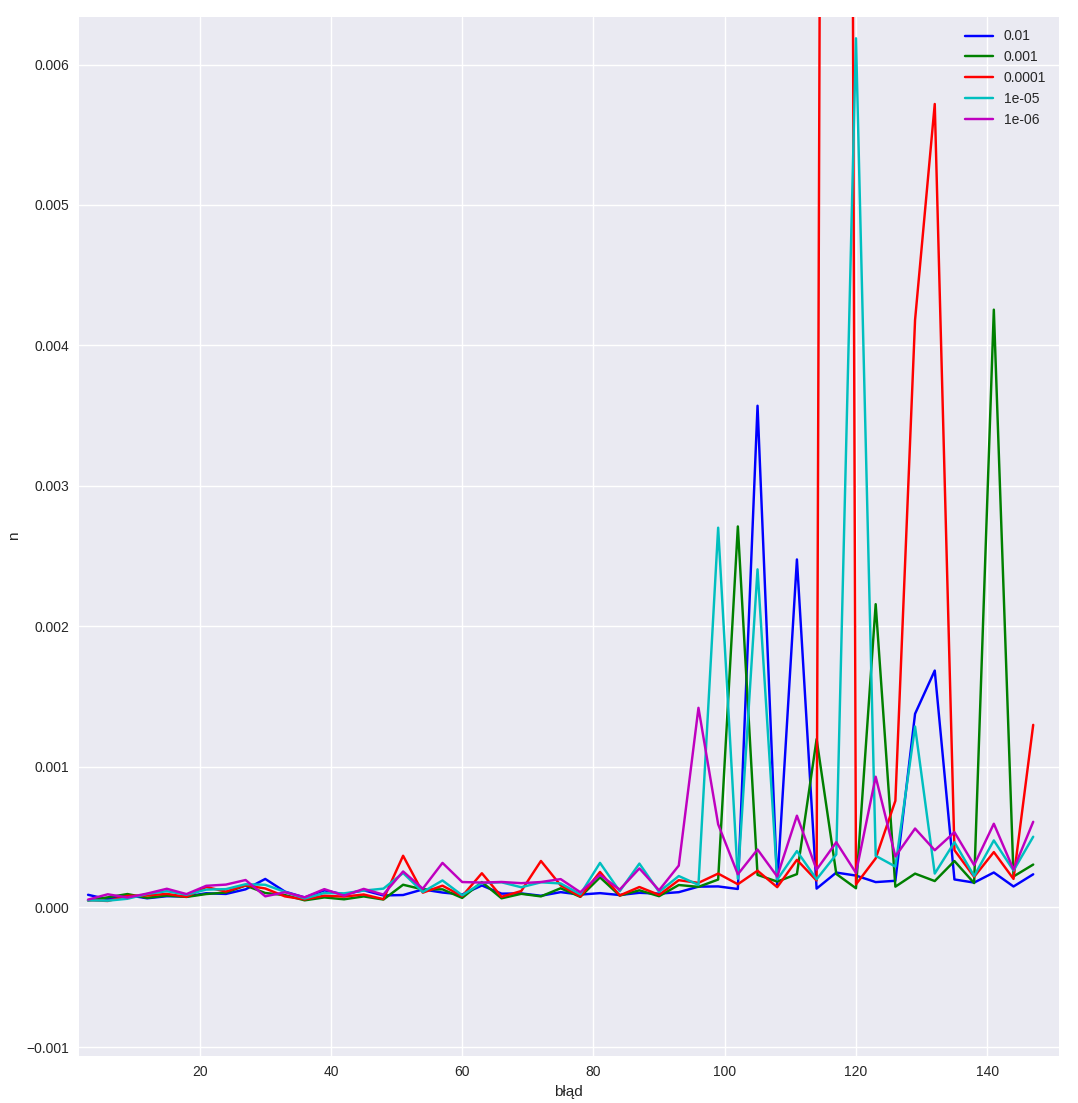
\includegraphics[width=\textwidth]{img/plot_5.png}
    \caption{Czas działania na podstawie powyższej tabeli}
\end{figure}

Czas działania jest bardzo niski (z pewnymi odstępstwami dla większych wartości $n$), co jest zasługą użycia operacji
macierzowych dostępnych w pakiecie numpy. W ogólności prezentuje on niewielką tendencję rosnącą z pewnymi nieregularnymi
skokami dla dużych wartości $n$, gdzie prezentują podobną tendencję jak w przypadku liczby iteracji. 
Efekt ten był jednak mocno uzależniony od próby.

\begin{table}[H]
\centering
\begin{tabular}{|l|l|l|l|l|l|}
\hline
& 0.01 & 0.001 & 0.0001 & 0.00001 & 0.000001 \\ \hline
3 & 0.0000885 & 0.0000448 & 0.0000405 & 0.0000460 & 0.0000520 \\ \hline
6 & 0.0000520 & 0.0000582 & 0.0000734 & 0.0000856 & 0.0000541 \\ \hline
9 & 0.0000689 & 0.0000970 & 0.0000622 & 0.0000677 & 0.0000753 \\ \hline
12 & 0.0000796 & 0.0000823 & 0.0000625 & 0.0000496 & 0.0000653 \\ \hline
15 & 0.0001304 & 0.0000694 & 0.0000732 & 0.0000966 & 0.0000982 \\ \hline
18 & 0.0000706 & 0.0000985 & 0.0000601 & 0.0000527 & 0.0000651 \\ \hline
21 & 0.0000758 & 0.0000951 & 0.0001533 & 0.0001709 & 0.0001230 \\ \hline
24 & 0.0000756 & 0.0001197 & 0.0001507 & 0.0001342 & 0.0000939 \\ \hline
27 & 0.0001285 & 0.0001628 & 0.0001502 & 0.0001769 & 0.0002279 \\ \hline
30 & 0.0001366 & 0.0001440 & 0.0001776 & 0.0001857 & 0.0000925 \\ \hline
33 & 0.0001054 & 0.0000894 & 0.0000973 & 0.0001476 & 0.0001600 \\ \hline
36 & 0.0000994 & 0.0000601 & 0.0000746 & 0.0000670 & 0.0001132 \\ \hline
39 & 0.0001359 & 0.0001042 & 0.0001075 & 0.0001552 & 0.0001526 \\ \hline
42 & 0.0001040 & 0.0000615 & 0.0000639 & 0.0001261 & 0.0000863 \\ \hline
45 & 0.0001435 & 0.0000920 & 0.0001085 & 0.0001378 & 0.0001724 \\ \hline
48 & 0.0001230 & 0.0000808 & 0.0001044 & 0.0001488 & 0.0001237 \\ \hline
51 & 0.0001485 & 0.0001559 & 0.0003209 & 0.0002754 & 0.0003614 \\ \hline
54 & 0.0001411 & 0.0000703 & 0.0000792 & 0.0001056 & 0.0001009 \\ \hline
57 & 0.0001059 & 0.0001199 & 0.0001338 & 0.0001545 & 0.0001893 \\ \hline
60 & 0.0000803 & 0.0000856 & 0.0000775 & 0.0000899 & 0.0001087 \\ \hline
63 & 0.0001833 & 0.0001509 & 0.0002174 & 0.0002193 & 0.0002525 \\ \hline
66 & 0.0001061 & 0.0000827 & 0.0001154 & 0.0001566 & 0.0001645 \\ \hline
69 & 0.0001287 & 0.0001419 & 0.0001631 & 0.0002213 & 0.0004468 \\ \hline
72 & 0.0000954 & 0.0000937 & 0.0000906 & 0.0001061 & 0.0001936 \\ \hline
75 & 0.0002260 & 0.0002913 & 0.0002909 & 0.0002234 & 0.0002582 \\ \hline
78 & 0.0001352 & 0.0001044 & 0.0001180 & 0.0001161 & 0.0001454 \\ \hline
81 & 0.0001812 & 0.0001636 & 0.0002263 & 0.0002744 & 0.0005000 \\ \hline
84 & 0.0001080 & 0.0001073 & 0.0001066 & 0.0001419 & 0.0001602 \\ \hline
87 & 0.0001502 & 0.0001736 & 0.0004206 & 0.0002897 & 0.0004199 \\ \hline
90 & 0.0001278 & 0.0002105 & 0.0001416 & 0.0001376 & 0.0001526 \\ \hline
93 & 0.0001891 & 0.0002127 & 0.0002286 & 0.0003140 & 0.0005865 \\ \hline
96 & 0.0001814 & 0.0003712 & 0.0001850 & 0.0001819 & 0.0002208 \\ \hline
99 & 0.0002198 & 0.0002406 & 0.0004840 & 0.0006256 & 0.0004938 \\ \hline
102 & 0.0001602 & 0.0001724 & 0.0001936 & 0.0009170 & 0.0002658 \\ \hline
105 & 0.0002341 & 0.0050430 & 0.0004256 & 0.0004683 & 0.0007200 \\ \hline
108 & 0.0024714 & 0.0001760 & 0.0002422 & 0.0051222 & 0.0004179 \\ \hline
111 & 0.0002668 & 0.0003059 & 0.0029092 & 0.0005157 & 0.0005651 \\ \hline
114 & 0.0032330 & 0.0001719 & 0.0002096 & 0.0025511 & 0.0003009 \\ \hline
117 & 0.0002780 & 0.0057919 & 0.0004408 & 0.0005164 & 0.0030587 \\ \hline
120 & 0.0001614 & 0.0001938 & 0.0024755 & 0.0002685 & 0.0002832 \\ \hline
123 & 0.0027502 & 0.0003624 & 0.0004699 & 0.0014372 & 0.0006979 \\ \hline
126 & 0.0001879 & 0.0026448 & 0.0002863 & 0.0002663 & 0.0017917 \\ \hline
129 & 0.0003397 & 0.0004182 & 0.0092058 & 0.0016429 & 0.0071719 \\ \hline
132 & 0.0062399 & 0.0548844 & 0.0002735 & 0.0003014 & 0.0003245 \\ \hline
135 & 0.0003462 & 0.0004387 & 0.0005884 & 0.0014827 & 0.0007622 \\ \hline
138 & 0.0002155 & 0.0002034 & 0.0002992 & 0.0012877 & 0.0004177 \\ \hline
141 & 0.0007682 & 0.0043020 & 0.0005875 & 0.0006642 & 0.0008454 \\ \hline
144 & 0.0002103 & 0.0002539 & 0.0006621 & 0.0010614 & 0.0003817 \\ \hline
147 & 0.0003996 & 0.0004659 & 0.0006325 & 0.0007353 & 0.0008531 \\ \hline
\end{tabular}
\caption{Czas (wiersze - $n$, kolumny - precyzja, kryterium stopu 2)}
\end{table}

Dla kryterium drugiego czasy działania są bardzo podobne, z bardzo nieznaczną przewagą czasową dla kryterium pierwszego.

\begin{figure}[H]
    \centering
    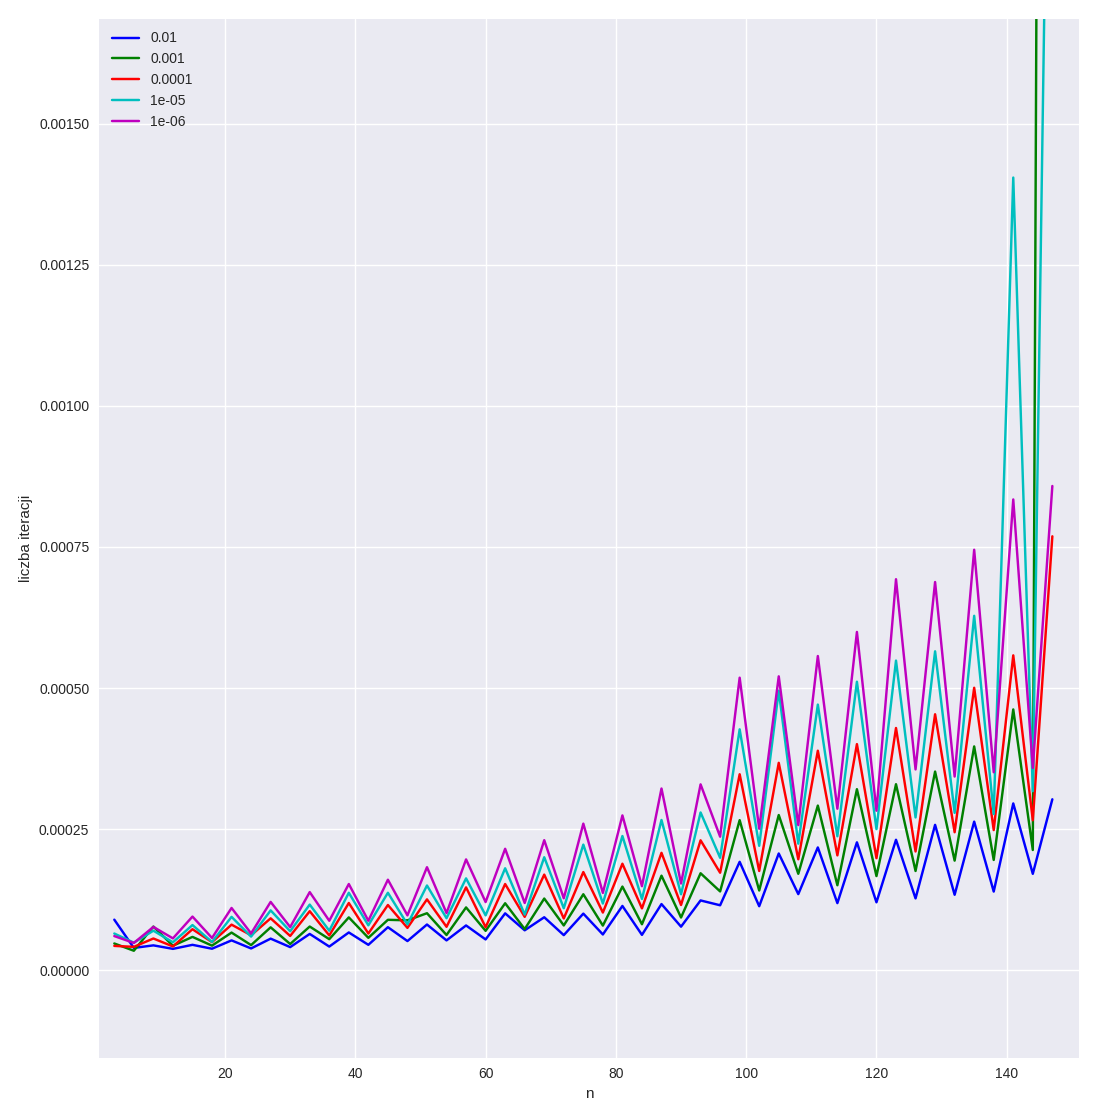
\includegraphics[width=\textwidth]{img/plot_6.png}
    \caption{Czas działania na podstawie powyższej tabeli}
\end{figure}

Teraz pozostaje zbadanie wpływu wektora początkowego. Tutaj zostanie użyte tylko kryterium pierwsze oraz precyzja $\rho=10^{-6}$. Użyte wektory
początkowe przyjmą postać \textbf{x}$\;=[a,a,...,a]$, gdzie $a$ będzie wartościami z zakresu $[-2,2]$.



\section{Problem 2}
\subsection{Opis problemu}
Przy użyciu dowolnej metody zostanie znaleziony promień spektralny macierzy iteracji z poprzedniego problemu
(dla różnych rozmiarów układu --- takich, dla których znajdowane były rozwiązania układu).
Sprawdzone zostanie, czy spełnione są założenia o zbieżności metody dla zadanego układu. Opisana zostanie metoda znajdowania
promienia spektralnego.

\subsection{Opracowanie problemu}
Promień spektralny jest wartością maksymalną spośród wartości bezwzględnych wartości własnych macierzy, tj.:
$$\rho(A)=max\{|\lambda_1|,..., |\lambda_n|\}$$
Wartościami własnymi macierzy nazywamy natomiast pierwiastki wielomianu charakterystycznego tej macierzy:
$$w_{A}(\lambda)=\det{A- \lambda I}$$
gdzie \textit{I} jest macierzą jednostkową. Do policzenia wartości własnych wielomianu użyta zostanie funkcja 
\textit{numpy.linalg.eigvals}.

Niech $\epsilon=x^{(t)}-x$, gdzie $x$ jest wektorem rzeczywistych rozwiązać układu równań. Wówczas macierz $M$ taką, że
$$\epsilon^{(t)}=M^t \cdot \epsilon^{(0)}$$
nazywamy macierzą iteracji.
Macierz iteracji dla metody Jakobiego ma postać
$$M=D^{-1}(L+U)$$
Gdzie (niech \textit{A} będzie macierzą układu równań)
$$A = D + L + U$$
\textit{D} jest macierzą diagonalną, z diagonalnych elementów macierzy \textit{A}, \textit{L} --- poddiagonalną, 
\textit{U} --- naddiagonalną. Mając te informację, można łatwo obliczyć promienie spektralne dla macierzy iteracji.

\newpage
\thispagestyle{empty}

\begin{table}[H]
\centering
\begin{tabular}{|l|l|}
\hline
$n$ & promień \\ \hline
3 & 0.05843 \\ \hline
4 & 0.08253 \\ \hline
5 & 0.10423 \\ \hline
6 & 0.12398 \\ \hline
7 & 0.14212 \\ \hline
8 & 0.15891 \\ \hline
9 & 0.17455 \\ \hline
10 & 0.18918 \\ \hline
11 & 0.20294 \\ \hline
12 & 0.21593 \\ \hline
13 & 0.22823 \\ \hline
14 & 0.23992 \\ \hline
15 & 0.25105 \\ \hline
16 & 0.26167 \\ \hline
17 & 0.27184 \\ \hline
18 & 0.28159 \\ \hline
19 & 0.29096 \\ \hline
20 & 0.29997 \\ \hline
21 & 0.30865 \\ \hline
22 & 0.31703 \\ \hline
23 & 0.32512 \\ \hline
24 & 0.33295 \\ \hline
25 & 0.34053 \\ \hline
26 & 0.34788 \\ \hline
27 & 0.35502 \\ \hline
28 & 0.36194 \\ \hline
29 & 0.36868 \\ \hline
30 & 0.37523 \\ \hline
31 & 0.38161 \\ \hline
32 & 0.38782 \\ \hline
33 & 0.39388 \\ \hline
34 & 0.39979 \\ \hline
35 & 0.40556 \\ \hline
36 & 0.41120 \\ \hline
37 & 0.41671 \\ \hline
38 & 0.42209 \\ \hline
39 & 0.42736 \\ \hline
40 & 0.43252 \\ \hline
41 & 0.43757 \\ \hline
42 & 0.44252 \\ \hline
43 & 0.44737 \\ \hline
44 & 0.45213 \\ \hline
45 & 0.45680 \\ \hline
46 & 0.46137 \\ \hline
47 & 0.46587 \\ \hline
48 & 0.47028 \\ \hline
49 & 0.47462 \\ \hline
50 & 0.47888 \\ \hline
51 & 0.48306 \\ \hline
\end{tabular}
\begin{tabular}{|l|l|}
\hline
$n$ & promień \\ \hline
52 & 0.48718 \\ \hline
53 & 0.49123 \\ \hline
54 & 0.49521 \\ \hline
55 & 0.49913 \\ \hline
56 & 0.50299 \\ \hline
57 & 0.50678 \\ \hline
58 & 0.51052 \\ \hline
59 & 0.51421 \\ \hline
60 & 0.51784 \\ \hline
61 & 0.52141 \\ \hline
62 & 0.52494 \\ \hline
63 & 0.52841 \\ \hline
64 & 0.53184 \\ \hline
65 & 0.53522 \\ \hline
66 & 0.53855 \\ \hline
67 & 0.54184 \\ \hline
68 & 0.54509 \\ \hline
69 & 0.54829 \\ \hline
70 & 0.55146 \\ \hline
71 & 0.55458 \\ \hline
72 & 0.55766 \\ \hline
73 & 0.56071 \\ \hline
74 & 0.56372 \\ \hline
75 & 0.56669 \\ \hline
76 & 0.56963 \\ \hline
77 & 0.57253 \\ \hline
78 & 0.57540 \\ \hline
79 & 0.57823 \\ \hline
80 & 0.58104 \\ \hline
81 & 0.58381 \\ \hline
82 & 0.58655 \\ \hline
83 & 0.58926 \\ \hline
84 & 0.59194 \\ \hline
85 & 0.59460 \\ \hline
86 & 0.59722 \\ \hline
87 & 0.59982 \\ \hline
88 & 0.60239 \\ \hline
89 & 0.60493 \\ \hline
90 & 0.60745 \\ \hline
91 & 0.60994 \\ \hline
92 & 0.61241 \\ \hline
93 & 0.61485 \\ \hline
94 & 0.61727 \\ \hline
95 & 0.61967 \\ \hline
96 & 0.62204 \\ \hline
97 & 0.62439 \\ \hline
98 & 0.62672 \\ \hline
99 & 0.62903 \\ \hline
100 & 0.63131 \\ \hline
\end{tabular}
\caption{Promienie spektralne}
\end{table}

Warunkiem wystarczającym zbieżności metody iteracyjnej jest
$$\rho(M)<1$$

Jak nietrudno zauważyć, dla wszystkich badanych wartości $n$ promień spektralny macierzy iteracji jest mniejszy
od jedynki, dla nich metoda jest zbieżna.

\subsection{Wnioski}


\end{document}